\documentclass{article}
\usepackage[utf8]{inputenc}
\usepackage[upright]{fourier} 
\usepackage{tikz, fullpage}
\usetikslibraray{ arrows, %
                  petri,  %
                topaths}
\usepackage{tkz-graph}
\begin{document}
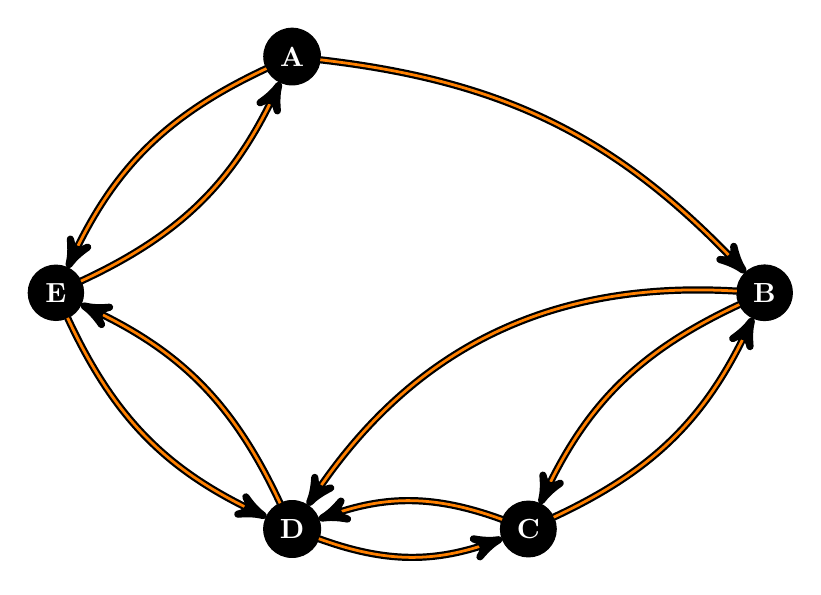
\begin{tikzpicture}[>=stealth']
    \SetGraphUnit{3}
    \tikzset{VertexStyle/.style = {shape        = circle,
                                   fill         = black,
                                   minimum size = 20pt,
                                   text         = white,
                                   draw}}
    \tikzset{TempStyle/.style = {double           = orange,
                                  double distance  = 1pt}}
    \Vertex[L = {\textbf{E}}]{E}
    \NOEA[  L = {\textbf{A}}](E){A}
    \SOEA[  L = {\textbf{D}}](E){D}
    \EA[    L = {\textbf{C}}](D){C}
    \NOEA[  L = {\textbf{B}}](C){B}
    \tikzset{EdgeStyle/.style = {TempStyle, 
                           ->,
                           bend right      = 20}}
    \Edges(A,E,D,C,B)
    \tikzset{EdgeStyle/.style = {TempStyle,
                                 ->,
                                 bend right      = 30}}
    \Edges(B,D)
    \tikzset{EdgeStyle/.style = {TempStyle, 
                                 <-,
                                 bend right      = 20}}
    \Edges(B,A) 
    \tikzset{EdgeStyle/.style = {TempStyle, 
                                 <-,
                                 bend left       = 20}}
    \Edges(A,E,D,C,B)
\end{tikzpicture}
\end{document}

